Anschließend werden die Messergebnisse der Laufzeit bei den verschiedenen Optimierung des Codes, sowie der Datenbankmanagement-Konfigurationen gezeigt.
Dabei wird unterschieden in Remote, also der lokalen Erstellung und externen Verarbeitung der Anfragen auf dem VM-DBMS oder Server (VM), der Erstellung und Verarbeitung der Anfragen lokal auf dem DBMS mit Docker-Einbindung.
\begin{figure}[h!]
    \center
    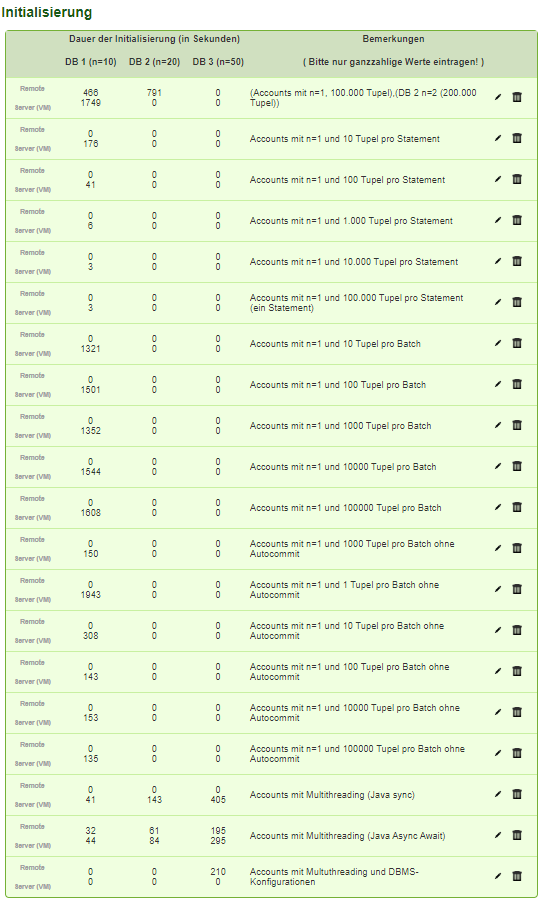
\includegraphics[width=\paperwidth/2]{assets/img/messungen}
    \caption{Messungen der Laufzeiten}
    \label{fig:messungen}
\end{figure}